
\newthought{Problem `Dutch National Flag'} in \textit{Programming, The Derivation of Algorithms}\cite{Kaldewaij90}.\index{Fibolucci}

\vspace{10 mm}
\begin{problem}
Write a program that swap elements of an array containing colors red, white and blue in such a way that the array's final state is in accordance with the Dutch National Flag. 
\end{problem}

\begin{marginfigure}

\includegraphics[scale=0.30]{flag.png}
\end{marginfigure}

This is a well known programming exercise used in many coding interviews. We will use it as an excuse to take a tour of the \textbf{weakest precondition calculus} also known as \textbf{wp-calculus} and the \textbf{Guarded Command Language} (\textbf{GCL}).

wp-calculus is part of the domain of Program Verification, Program Construction and Refinement calculus. There was an effort in the computer science community in the 1970's, 1980's and 1990's to develop a logical framework for the formal derivation of programs.

  
To keep this tour short we are going to take a pretty informal\footnote{We won't define program state, program execution and variables. We will convey the meaning of these concepts through examples. We will use integer and boolean operators, predicate calculus and quantified expressions in the usual way.} approach that hopefully still captures the essence of wp-calculus. We start with a boolean expression called \textbf{Hoare triple}: $\{P\} S \{R\}$. $P$ and $R$ are logical predicates asserting something about the state of some program execution. $S$ is a program statement that may or may not terminate. The Hoare triple $\{P\} S \{R\}$ states that executing $S$ in a programming state where $P$ is true guarantees that $R$ is true afterwards if the execution of $S$ terminates. The Hoare triple doesn't say anything about the value of $R$ if $P$ is false, $R$ could be true or false. It also doesn't say anything about the value of $R$ if $S$ does not terminate. The relationship between $P$ and $R$ is not unique: given $S$ and $R$ there can be many $P$ satisfying $\{P\} S \{R\}$ and given $P$ and $S$ there can be many $R$ satisfying $\{P\} S \{R\}$.

\begin{marginfigure}
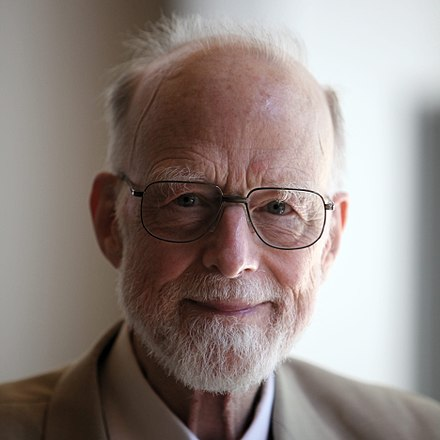
\includegraphics[scale=0.33]{hoare.jpg}
\end{marginfigure}
\marginnote{Sir Charles Antony Richard Hoare is one of the giants of computer science, inventor of Quicksort and Hoare Logic of which the Hoare triple is a key feature. \url{https://en.wikipedia.org/wiki/Tony_Hoare}}

Let's look at some examples. Given the following $R$ and $S$

\begin{align*}
R &: x > 0 \\
S &: x := x - 1
\end{align*}

the Hoare triples $\{x = 20\} x := x - 1 \{x > 0\}$, $\{x > 5\} x := x - 1 \{x > 0\}$ and $\{x > 0\} x := x - 1 \{x > 0\}$ are all true. On the other hand $\{x = 0\} x := x - 1 \{x > 0\}$ is false.

Not requiring $S$ to terminate and not having unique relationships between $P$ and $R$ makes it harder to reason about the correctness of a program. To remedy this Edsger W. Dijkstra introduced wp-calculus: given statement $S$ and postcondition $R$ we say $wp.S.R$ is the weakest precondition such that the Hoare triple $\{wp.S.R\} S \{R\}$ holds and $S$ terminates\footnote{
\bibentry{Dijkstra75}\\
 This paper introduced the wp-calculus and the Guarded Command Language.
}. 

\begin{marginfigure}

\includegraphics[scale=0.6]{dijkstra.png}
\end{marginfigure}
\marginnote{Edsger W. Dijkstra, another giant of computer science, famous for the shortest path in a graph algorithm, among many other things. \url{https://en.wikipedia.org/wiki/Edsger_W._Dijkstra}}

We mean by weakest the most general, least restrictive precondition, i.e. if $A$ and $B$ are two predicates and $A \implies B \wedge \lnot (B \implies A)$ then $B$ is weaker than $A$. We note that $wp$ is a function that given statement $S$ maps predicate $R$ to predicate $P$ and for a given $R$ the predicate $P$ is unique. For this reason $wp$ is a predicate transformer. We use the dot notation for function application, so $f.x.y$ is the same as $f(x, y)$ in classical mathematical notation. The dot notation makes separating the arguments more readable and avoids confusion about where $S$ terminates and $R$ starts.
 

With a given postcondition as our goal of what a program should do, wp-calculus let's us go backwards and calculate the necessary statements and preconditions to achieve this desired postcondition goal. In doing so we also prove that the calculated program is correct.

To illustrate this we need to bring in the Guarded Command Language that let's us specify programs and for each statement type in this language define axiomatically what the $wp$ function is. We will do this for assignment statements, sequential composition, if-statements and loops. We will also do a special axiom useful for the Dutch National Flag problem involving a swapping of array elements statement.

\begin{defn}
The weakest precondition of the \textbf{assignment statement} $x := E$ is 
$$
(wp.x := E.R) \equiv R[x \leftarrow E] 
$$

where $R[x \leftarrow E]$ denotes the predicate obtained from $R$ with all free occurrences\footnote{The distinction between free and bound occurrences of a variable $x$ is necessary if a boolean predicate has a boolean quantified subexpression using $x$ in a bound way, for example the subexpression $\{\forall x \in A: x^2 - 1\}$. We will avoid this confusion in this exposition by choosing our variable names carefully.} of $x$ substituted by $E$.
\end{defn}


